\documentclass[12pt]{article}  
%%Read the manual for other options. 

\pagestyle{empty} %%Eliminates page numbers
%%\input rmb_macros
%%Collect your favorite macros in a 
%%separate file

%\input amssym.def
%\input amssym
%\input mssymb
%%Defines additional symbols



\usepackage{graphics}
\usepackage{amsmath,amssymb,amsthm, multicol,mathtools}
\usepackage[pdftex]{graphicx}
\usepackage{epsf}
%%Use to include pictures. 

%\newcommand{\comment}[1]{}
%\newcommand{\sobolev}[2]{W^{#1,#2}}
%\newcommand{\sobolev}[2]{L^#2_#1}
%%Some examples of macros or new commands.

\addtolength{\oddsidemargin}{-.75in}
\addtolength{\evensidemargin}{-.75in}
\addtolength{\textwidth}{1.5in}
\addtolength{\topmargin}{-1in}
\addtolength{\textheight}{2.25in}
%%Set margins, defaults are ok. 

\begin{document}
\begin{center}
{\bf \Large Eigenvalues and Eigenvectors}
\vspace{0.2cm}
\hrule
\end{center}

\begin{multicols*}{2}
	\begin{enumerate}
		\item Is $\lambda = -3$ an eigenvalue of $\begin{bmatrix*}[r]
			-1 & 4\\ 6 & 9
		\end{bmatrix*}$?

		\vfill

		\item Is $\begin{bmatrix*}[r]
			1\\-2\\2
		\end{bmatrix*}$ an eigenvector of $\begin{bmatrix}
			3&6&7\\ 3&2&7\\ 5&6&4
		\end{bmatrix}$? If so, find the eigenvalue.

		\vfill

		\item Find a basis for the eigenspace corresponding to each listed eigenvalue.
		\begin{enumerate}
			\item $A = \begin{bmatrix*}[r]
				4 & 1\\3&6
			\end{bmatrix*}$, $\lambda = 3, 7$.
			\vfill
			\item $A=\begin{bmatrix*}[r]
				4&0&-1\\ 3&0&3\\ 2&-2&5
			\end{bmatrix*}$, $\lambda = 3$.
		\end{enumerate}

		\vfill\null\columnbreak

		\item Let $u$ and $v$ be the vectors shown in the figure and suppose that $u$ and $v$ are eigenvectors of a $2\times 2$ matrix $A$ that correspond to eigenvalues 2 and 3, respectively. Let $T:\mathbb{R}^2\to \mathbb{R}^2$ be the linear transformation given by $T(x) = Ax$, and let $w=u+v$. Make a copy of the figure and on the same set of axes, plot $T(u)$, $T(v)$, and $T(w)$.\\
		\centerline{
		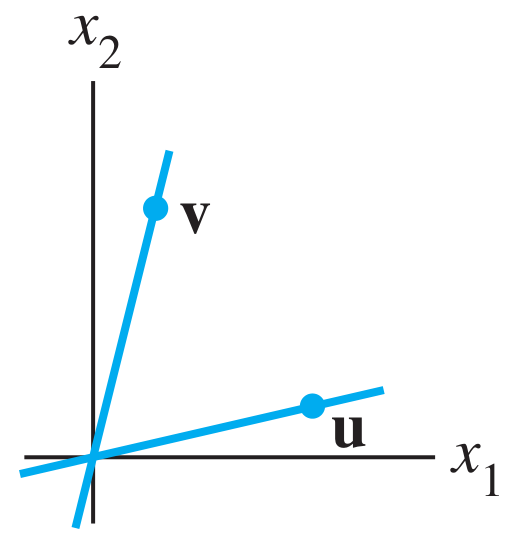
\includegraphics[scale=.3]{graph.PNG}}
		\vfill

		\item Find the characteristic polynomial and the eigenvalues of the matrices.
		\begin{enumerate}
			\item $\begin{bmatrix*}[r]
				-4&-1\\6&1
			\end{bmatrix*},\quad\text{(b)}\quad
			\begin{bmatrix*}[r]
				9 & -2\\
				2&5
			\end{bmatrix*}
			$
		\end{enumerate}
		\vfill

		\item Find the characteristic polynomial
		\[
		\begin{bmatrix*}[r]
			3&1&1\\
			0&5&0\\
			-2&0&7
		\end{bmatrix*}
		\]
		\vfill

		\item List the eigenvalues along with their algebraic multiplicities.
		\[
		\begin{bmatrix*}[r]
			3&0&0&0\\
			6&2&0&0\\
			0&3&6&0\\
			2&3&3&-5
		\end{bmatrix*}
		\]
		\vfill
	\end{enumerate}
\end{multicols*}
%Section 5.1: 1-19 odd, 21, 22, 23, 24, 25, 26, 31, 32

%Section 5.2: 1-17 odd, 19, 20, 21, 22, 23, 24

\end{document}